\documentclass{article}
\usepackage[utf8]{inputenc}
\usepackage{graphicx}


\title{RENTAL FILM}
\author{yukiardiansyah321 }
\date{December 2019}

\begin{document}

\maketitle

\section{Pembuatan Table Dan view }

\begin{enumerate}
    \item langkah pertama dalam pembuatan aplikasi baru di apex online adalah membuka menu tampilan apex oracle di aplikasi pencarian yang ada buka apex oracle expres dan login
    
    \begin{center}
         \centering
            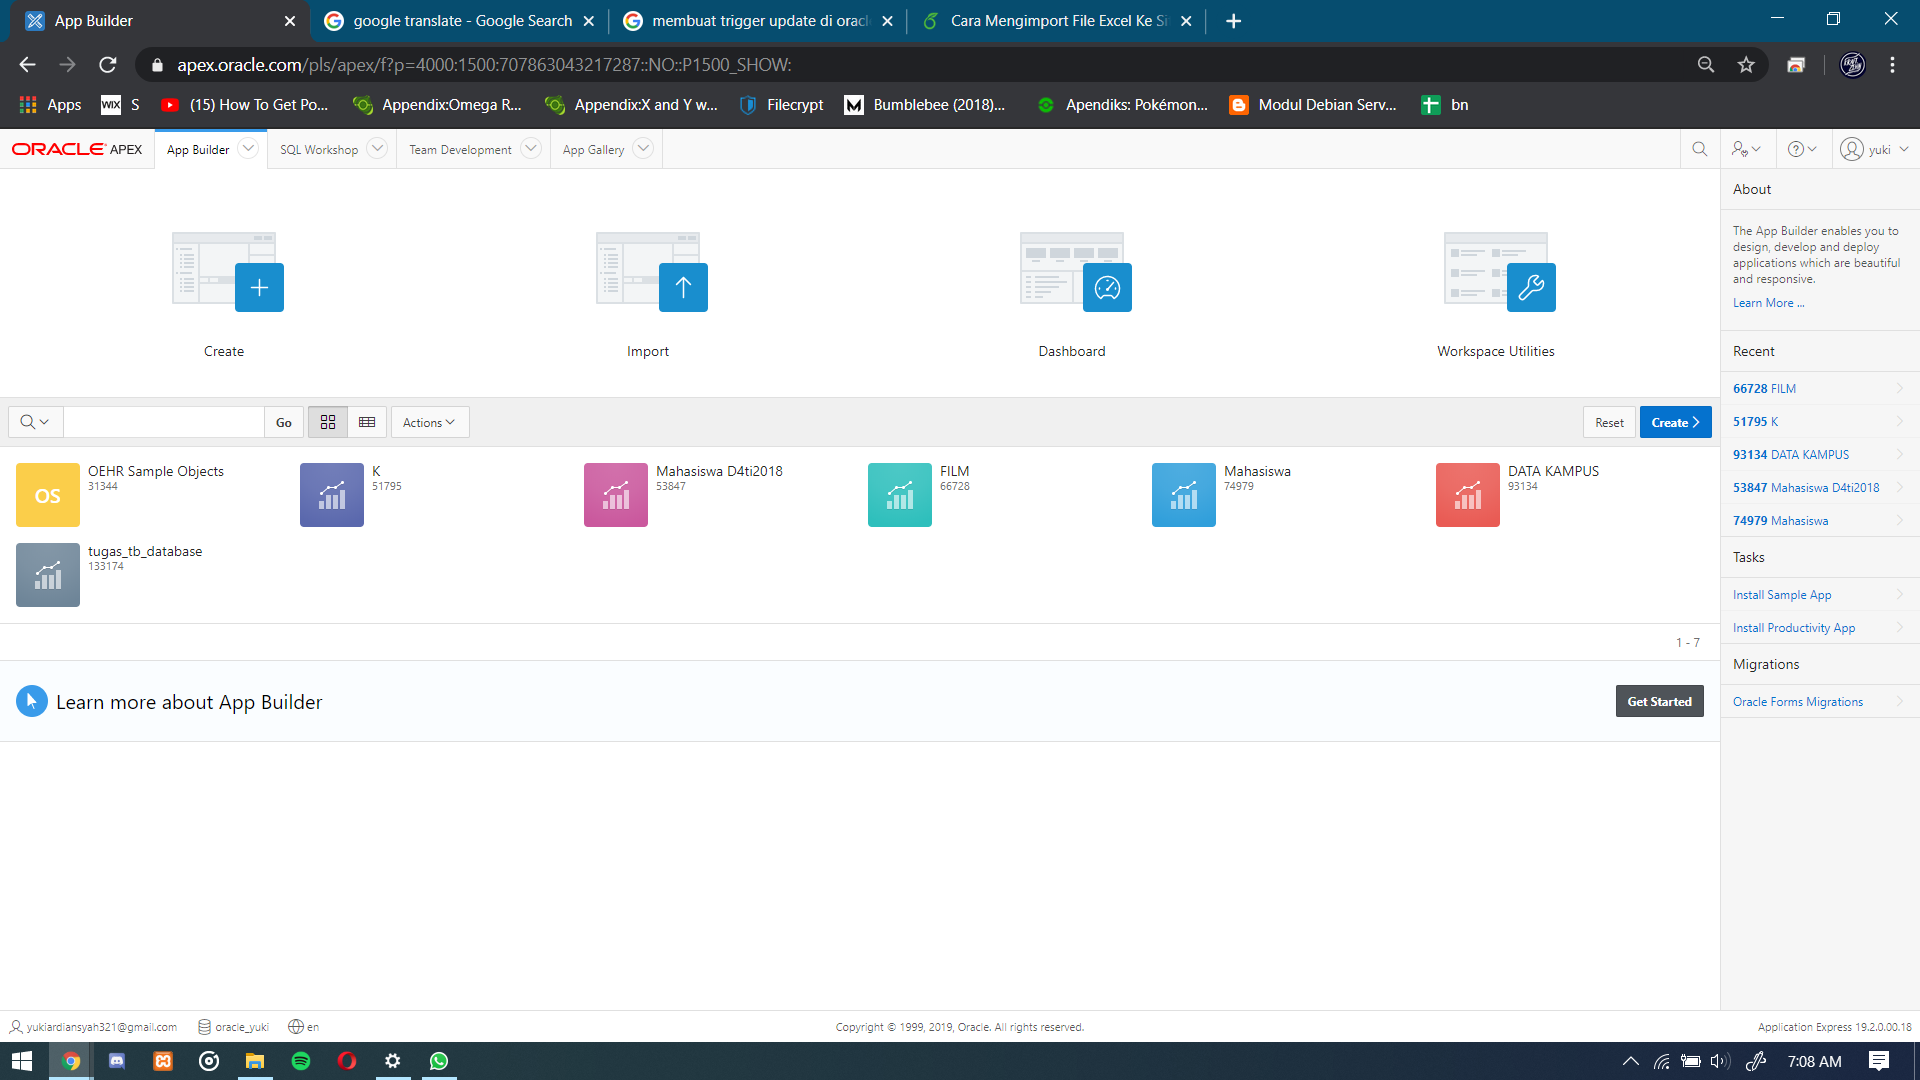
\includegraphics[scale=0.27]{figures/0.PNG}
        \caption{Menu Aplikasi apex}
        \label{excel}
    \end{center}
       
     \item setelah itu buka object command untuk melakukan perintah seperti membuat table menambahkan
     primary key, foreign key dan insert trigger atau view
      
    \begin{center}
         \centering
            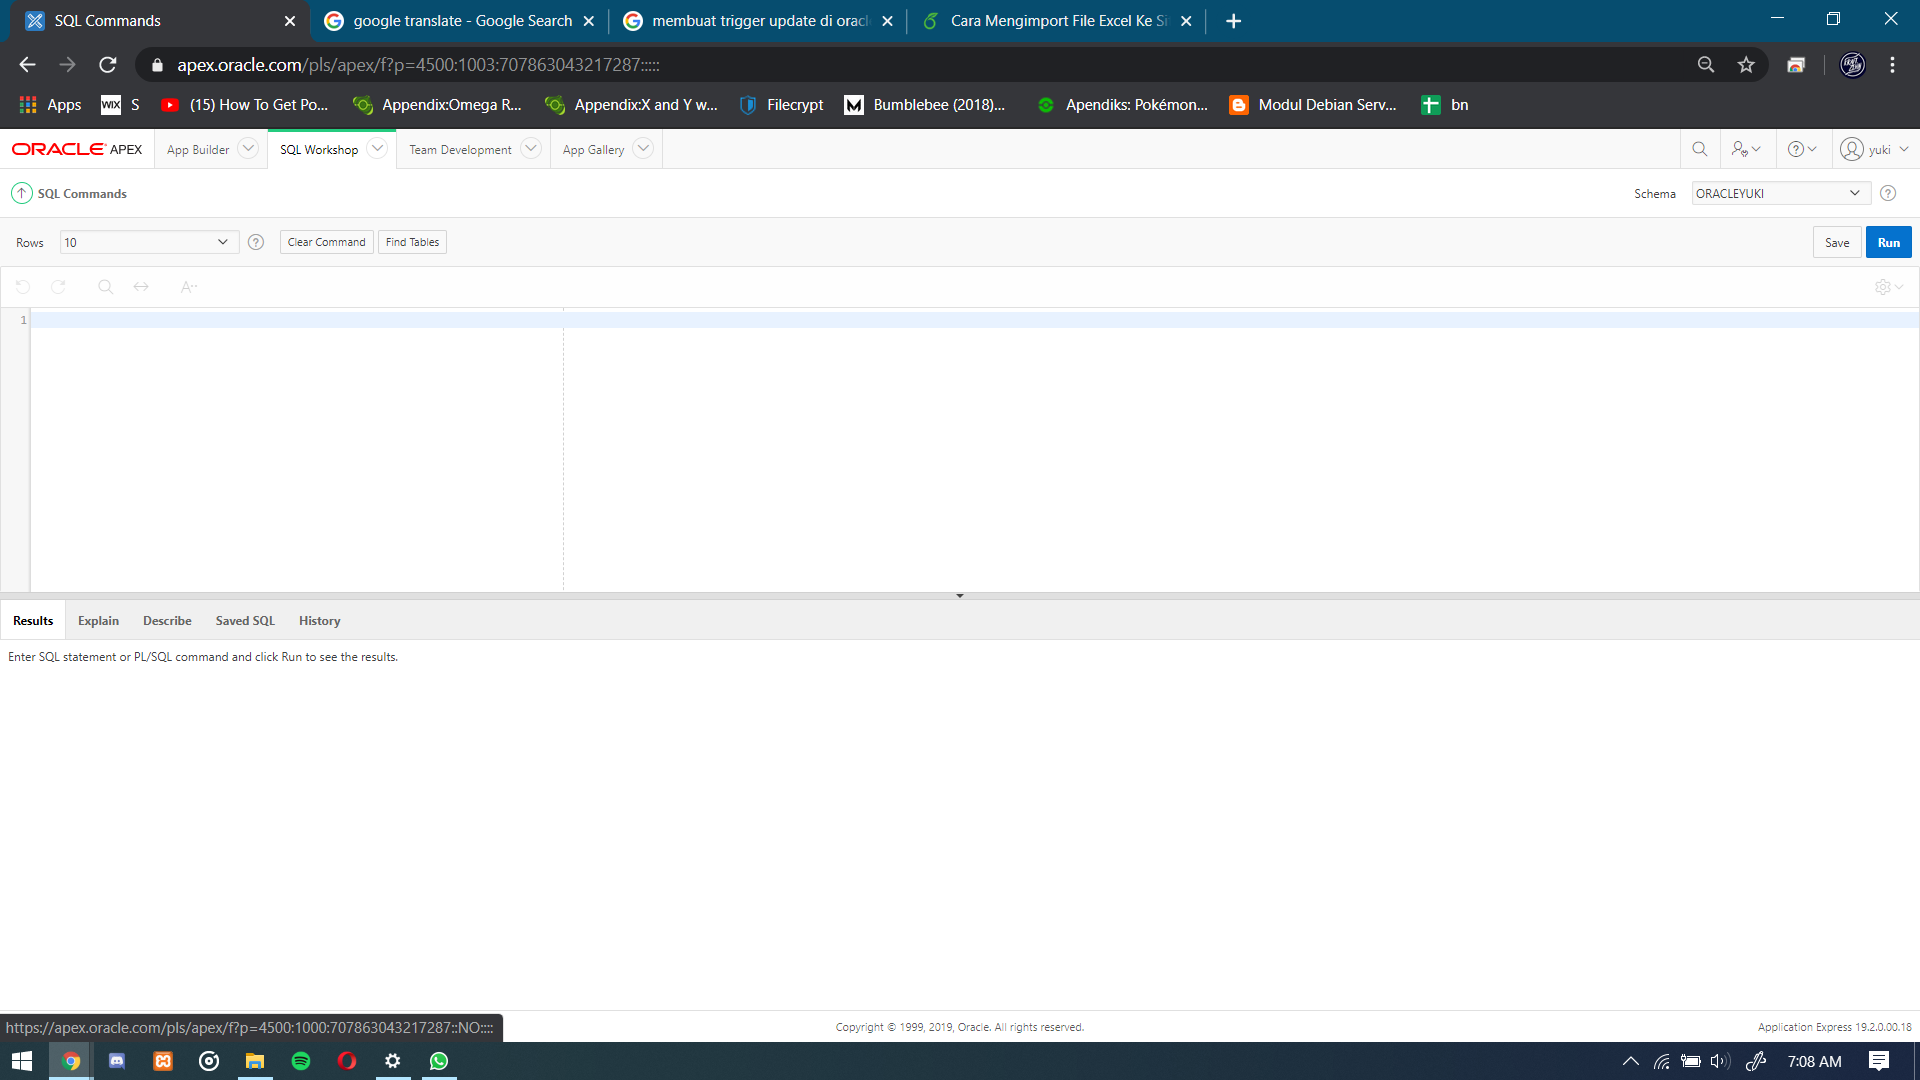
\includegraphics[scale=0.27]{figures/8.PNG}
        \caption{Command }
        \label{create}
    \end{center}
    
    \item langkah pertama membuat table dari film yang akan di rental dengan values seperti gambar di bawah
      
    \begin{center}
         \centering
            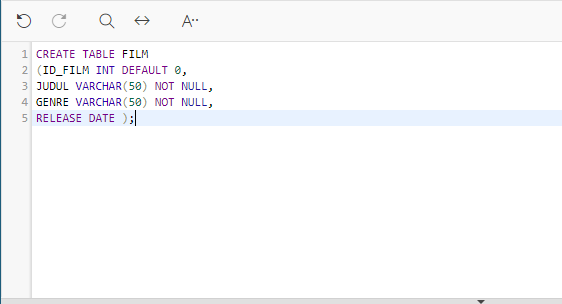
\includegraphics[scale=0.27]{figures/1.PNG}
        \caption{membuat table }
        \label{create}
    \end{center}
    
     \item selanjutnya membuat table menu dari pemimjaman film yang akan dibuat
      
    \begin{center}
         \centering
            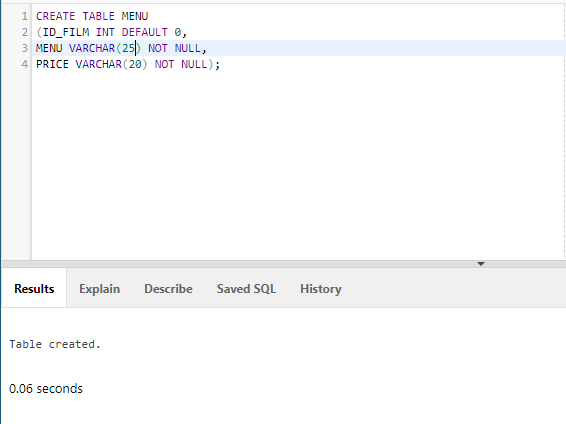
\includegraphics[scale=0.27]{figures/2.PNG}
        \caption{membuat table menu }
        \label{create}
    \end{center}
    
     \item setelah itu membuat table transaction untuk melihat hasil transaksi dari peminjaman film
      
    \begin{center}
         \centering
            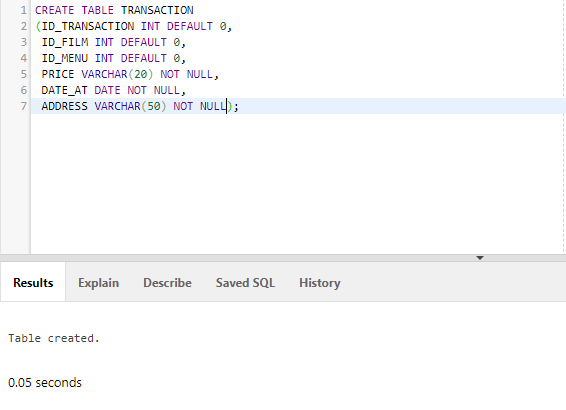
\includegraphics[scale=0.27]{figures/3.PNG}
        \caption{membuat table transaction }
        \label{create}
    \end{center}
    
     \item langkah selanjutnya dengan menbuat primary key dari setiap table yang telah kita buat
    \begin{center}
         \centering
            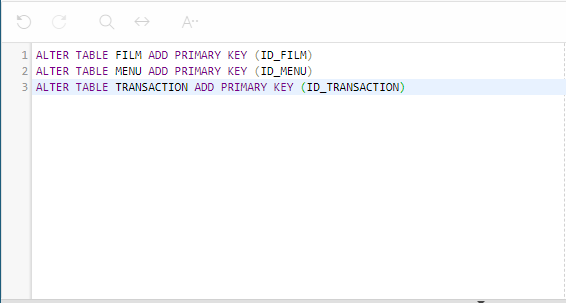
\includegraphics[scale=0.27]{figures/4.PNG}
        \caption{primary key }
        \label{create}
    \end{center}
    
    \item setelah itu kita membuat foreign key agar table - table yang telah kita buat berlerasi dengan table yang lainnya
    \begin{center}
         \centering
            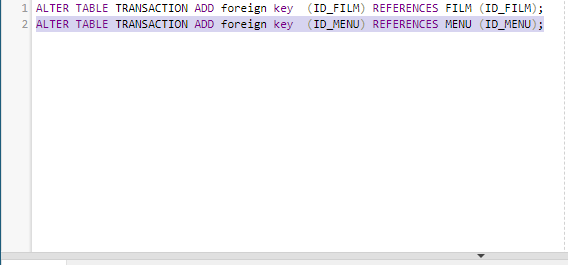
\includegraphics[scale=0.27]{figures/5.PNG}
        \caption{foreign key }
        \label{create}
    \end{center}
    
    \item untuk melihat apa table sudah berlerasi bisa dilihat melalui klik tablenya dan buka menu models
    \begin{center}
         \centering
            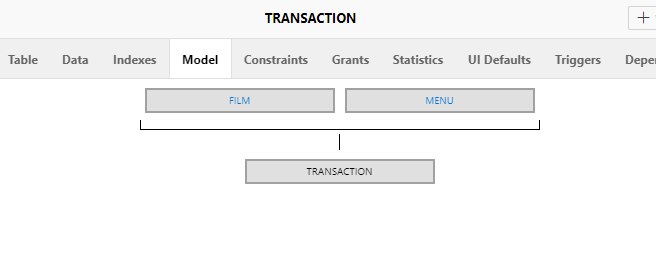
\includegraphics[scale=0.27]{figures/6.PNG}
        \caption{relasi }
        \label{create}
    \end{center}
    
    \item setelah itu masukan values dari setiap table dengan melakukan command insert ke setiap table sebagai berikut
    \begin{center}
         \centering
            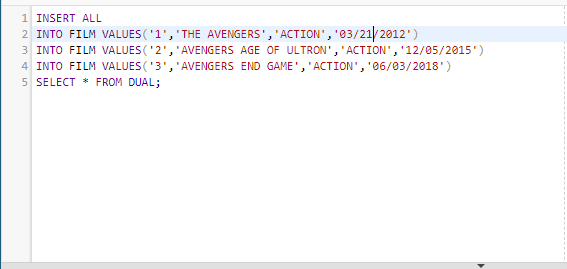
\includegraphics[scale=0.27]{figures/7.PNG}
        \caption{insert }
        \label{create}
    \end{center}
    
    \item setelah itu membuat sebuah trigger insert dan update di dalam table film dan menu
    \begin{center}
         \centering
            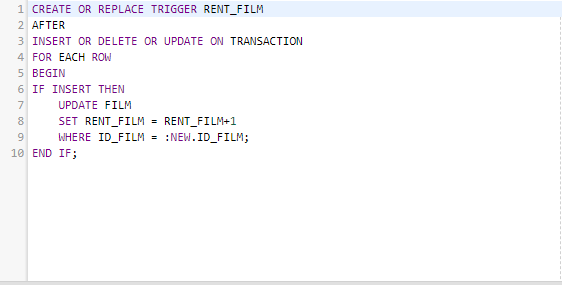
\includegraphics[scale=0.27]{figures/9.PNG}
        \caption{trigger }
        \label{create}
    \end{center}
      
    
\end{enumerate}

\section{Membuat Aplikasi Rental Film}
\begin{enumerate}
    \item langkah pertama adalah klik app builder dan klik create
    
    \begin{center}
         \centering
            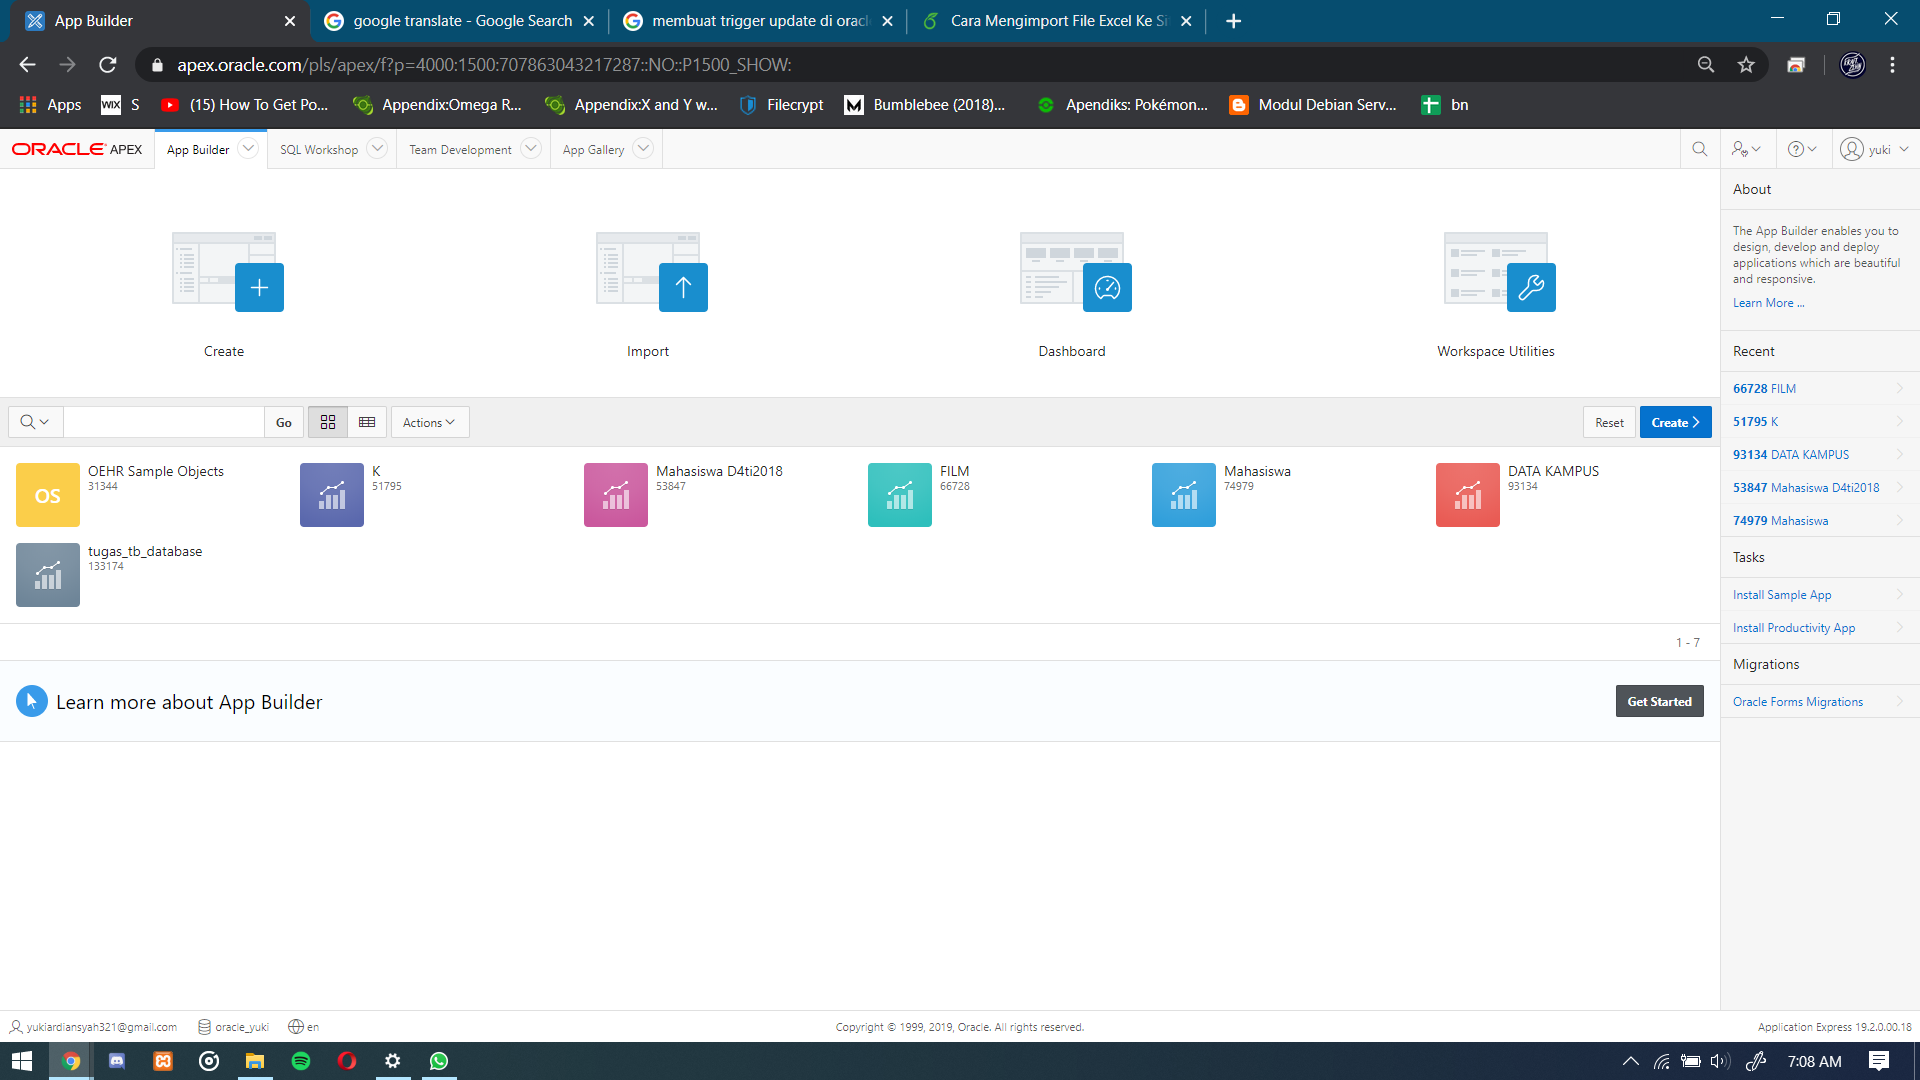
\includegraphics[scale=0.27]{figures/0.PNG}
        \caption{Menu Aplikasi apex}
    \end{center}
    
      \item setelah memilih menu create selanjutnya pilih menu new application untuk
membuat aplikasi baru.
    
    \begin{center}
         \centering
            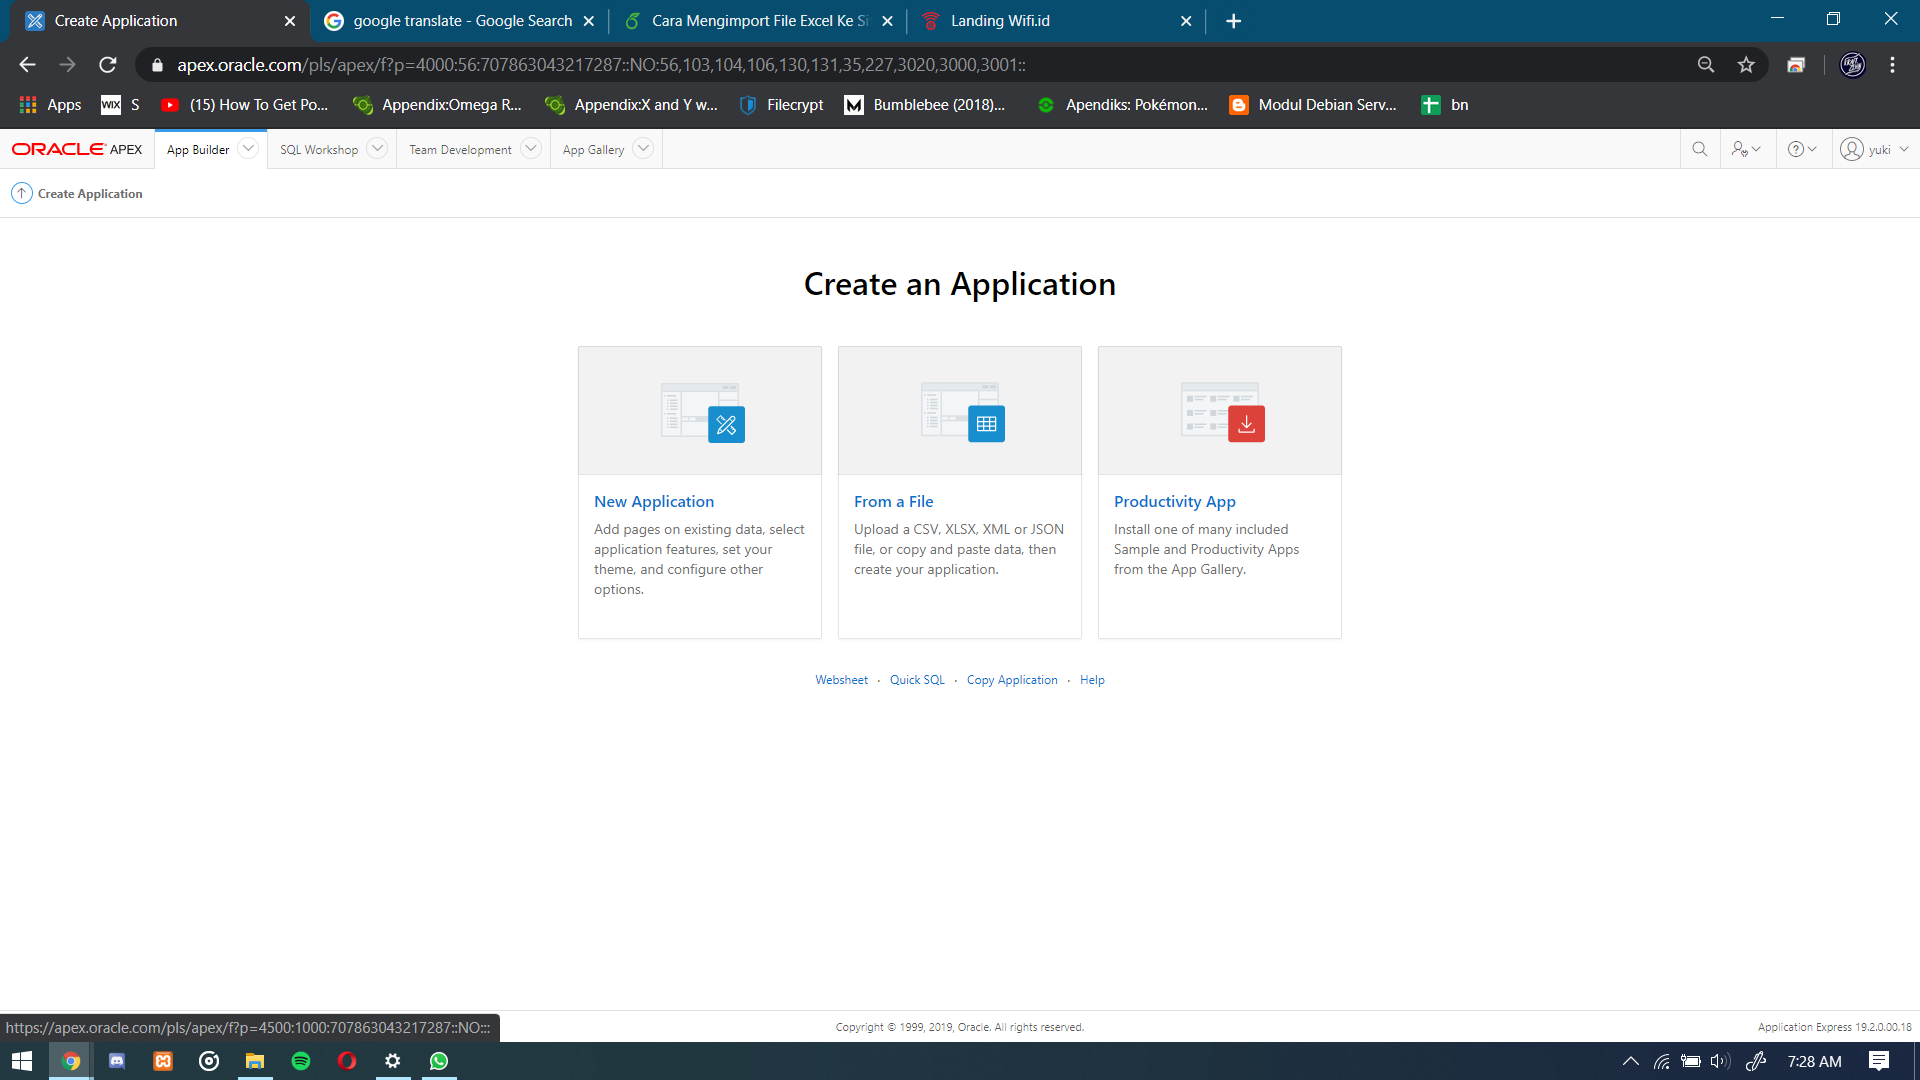
\includegraphics[scale=0.27]{figures/10.PNG}
        \caption{Menu create}
    \end{center}

\item setelah itu membuat nama aplikasi sesuai yang telah dibuat
    
    \begin{center}
         \centering
            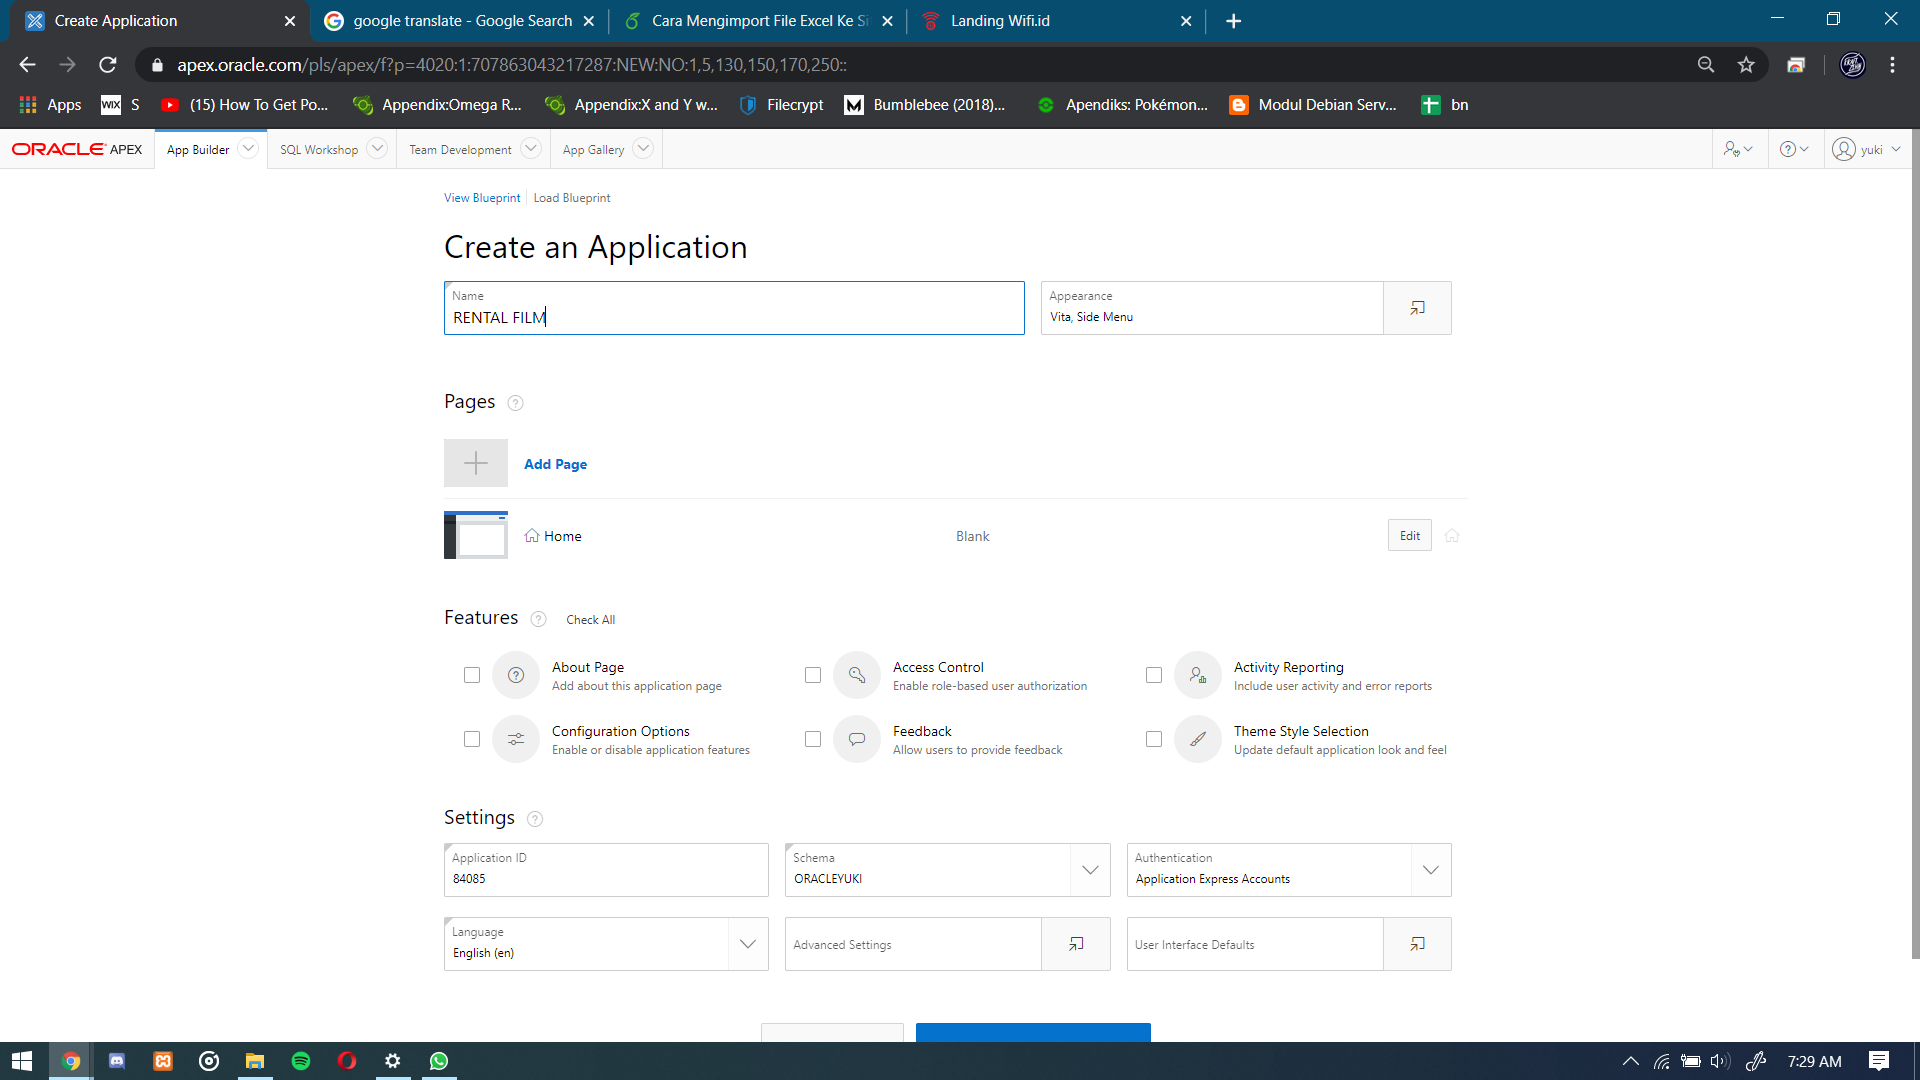
\includegraphics[scale=0.27]{figures/11.PNG}
        \caption{Menu name}
    \end{center}
    
    \item setelah nama aplikasi telah dibuat selanjutnya membuat menu pada aplikasi
dengan add page .disini kita memilih menu interactive menu.
    
    \begin{center}
         \centering
            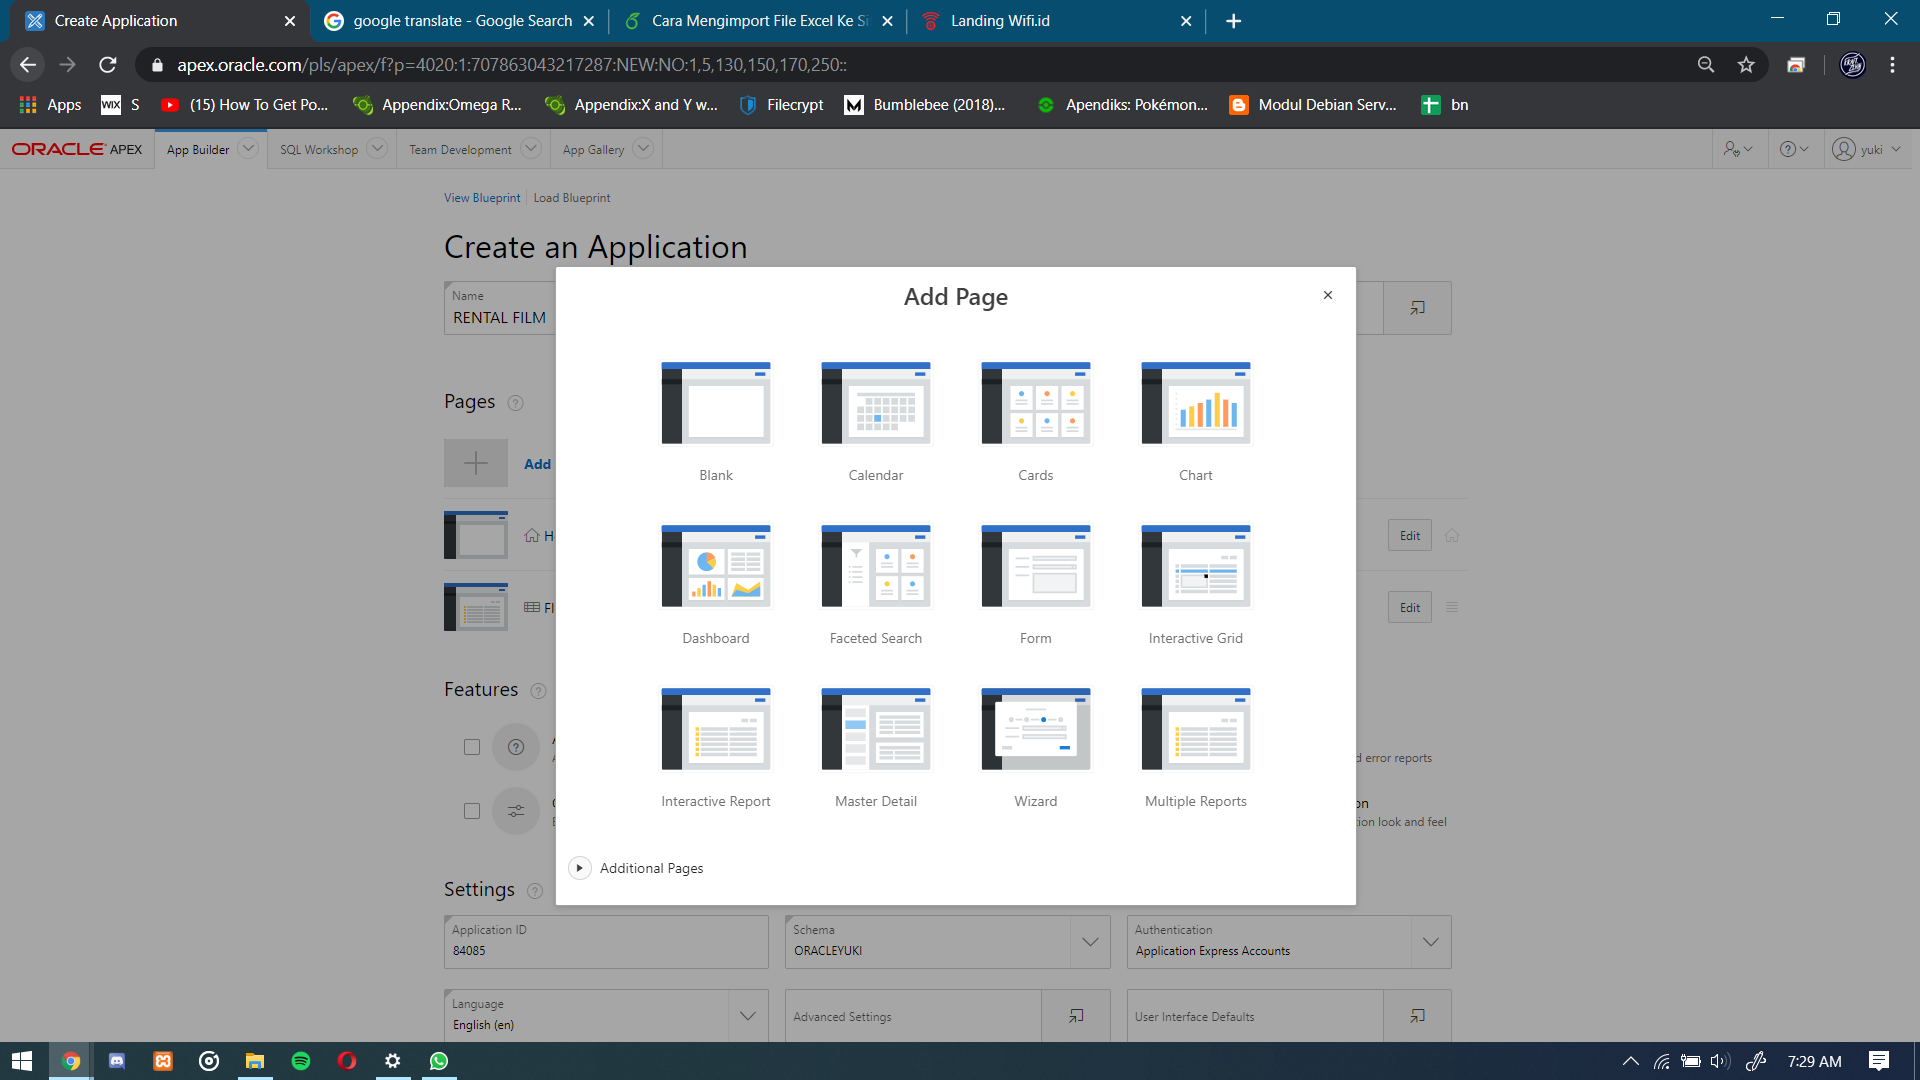
\includegraphics[scale=0.27]{figures/12.PNG}
        \caption{Menu add page}
    \end{center}


\item setelah Add page kita menamai page name dan menambahkan table sesuai name page. lakukan hal yang sama dengan table yang lainnya
    
    \begin{center}
         \centering
            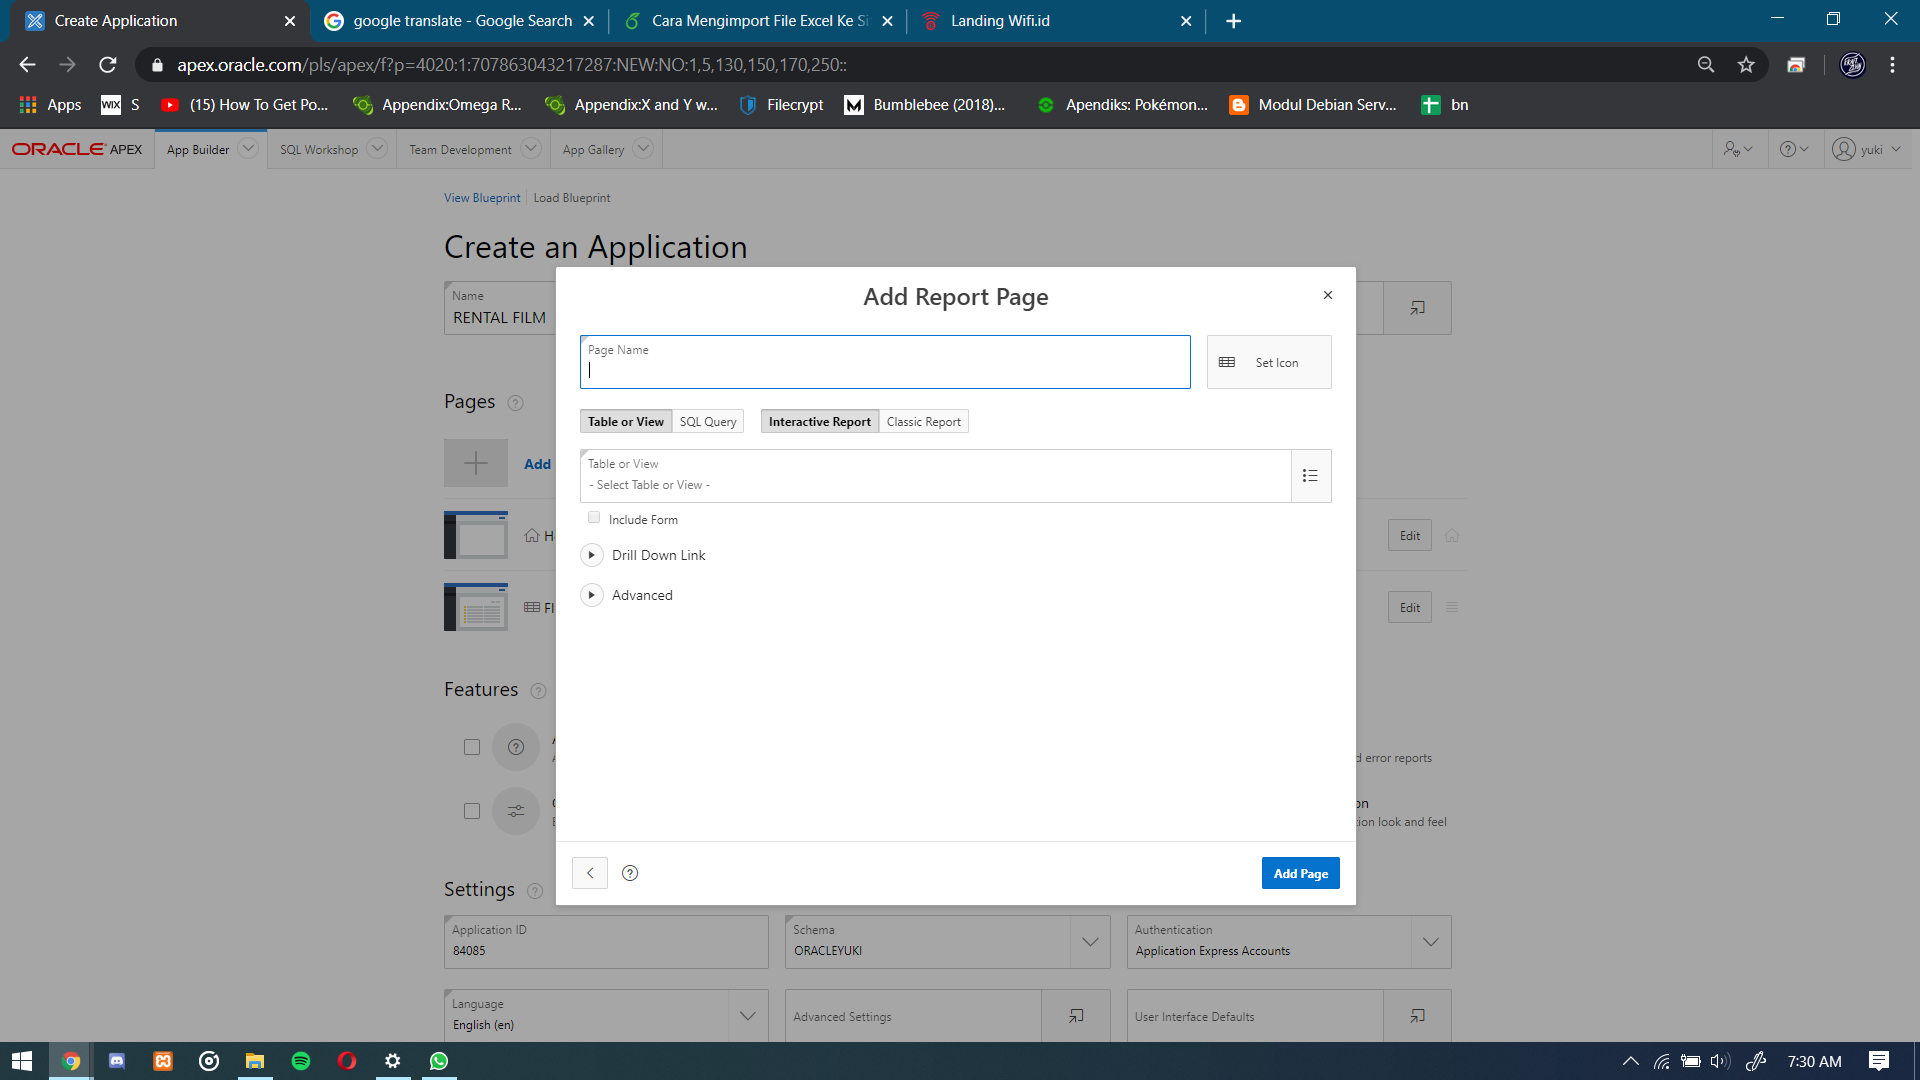
\includegraphics[scale=0.27]{figures/13.PNG}
        \caption{Menu add table}
    \end{center}
    
    \item Masukkan Passsword Dan Username
    \begin{center}
         \centering
            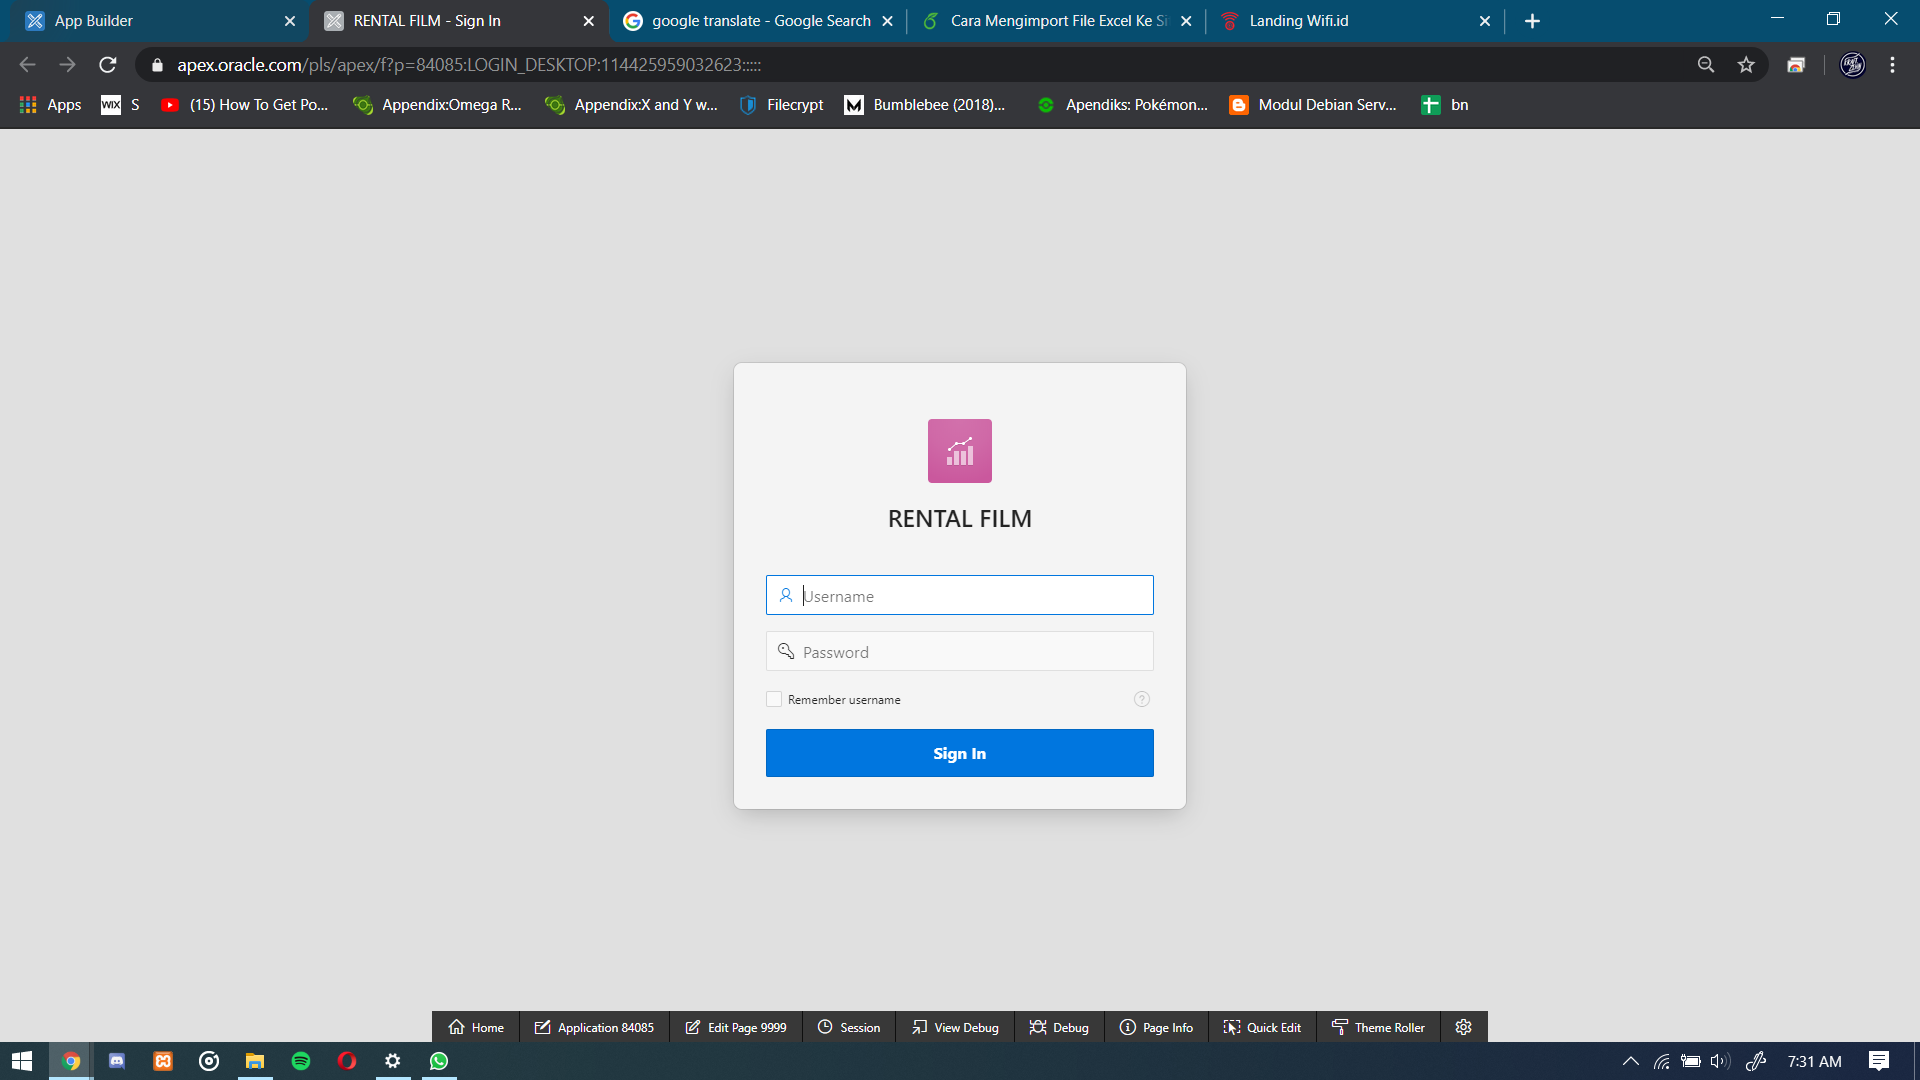
\includegraphics[scale=0.27]{figures/14.PNG}
        \caption{Masukkan Password}
    \end{center}
    
    \item setelah itu aplikasi siap digunakan
    \begin{center}
         \centering
            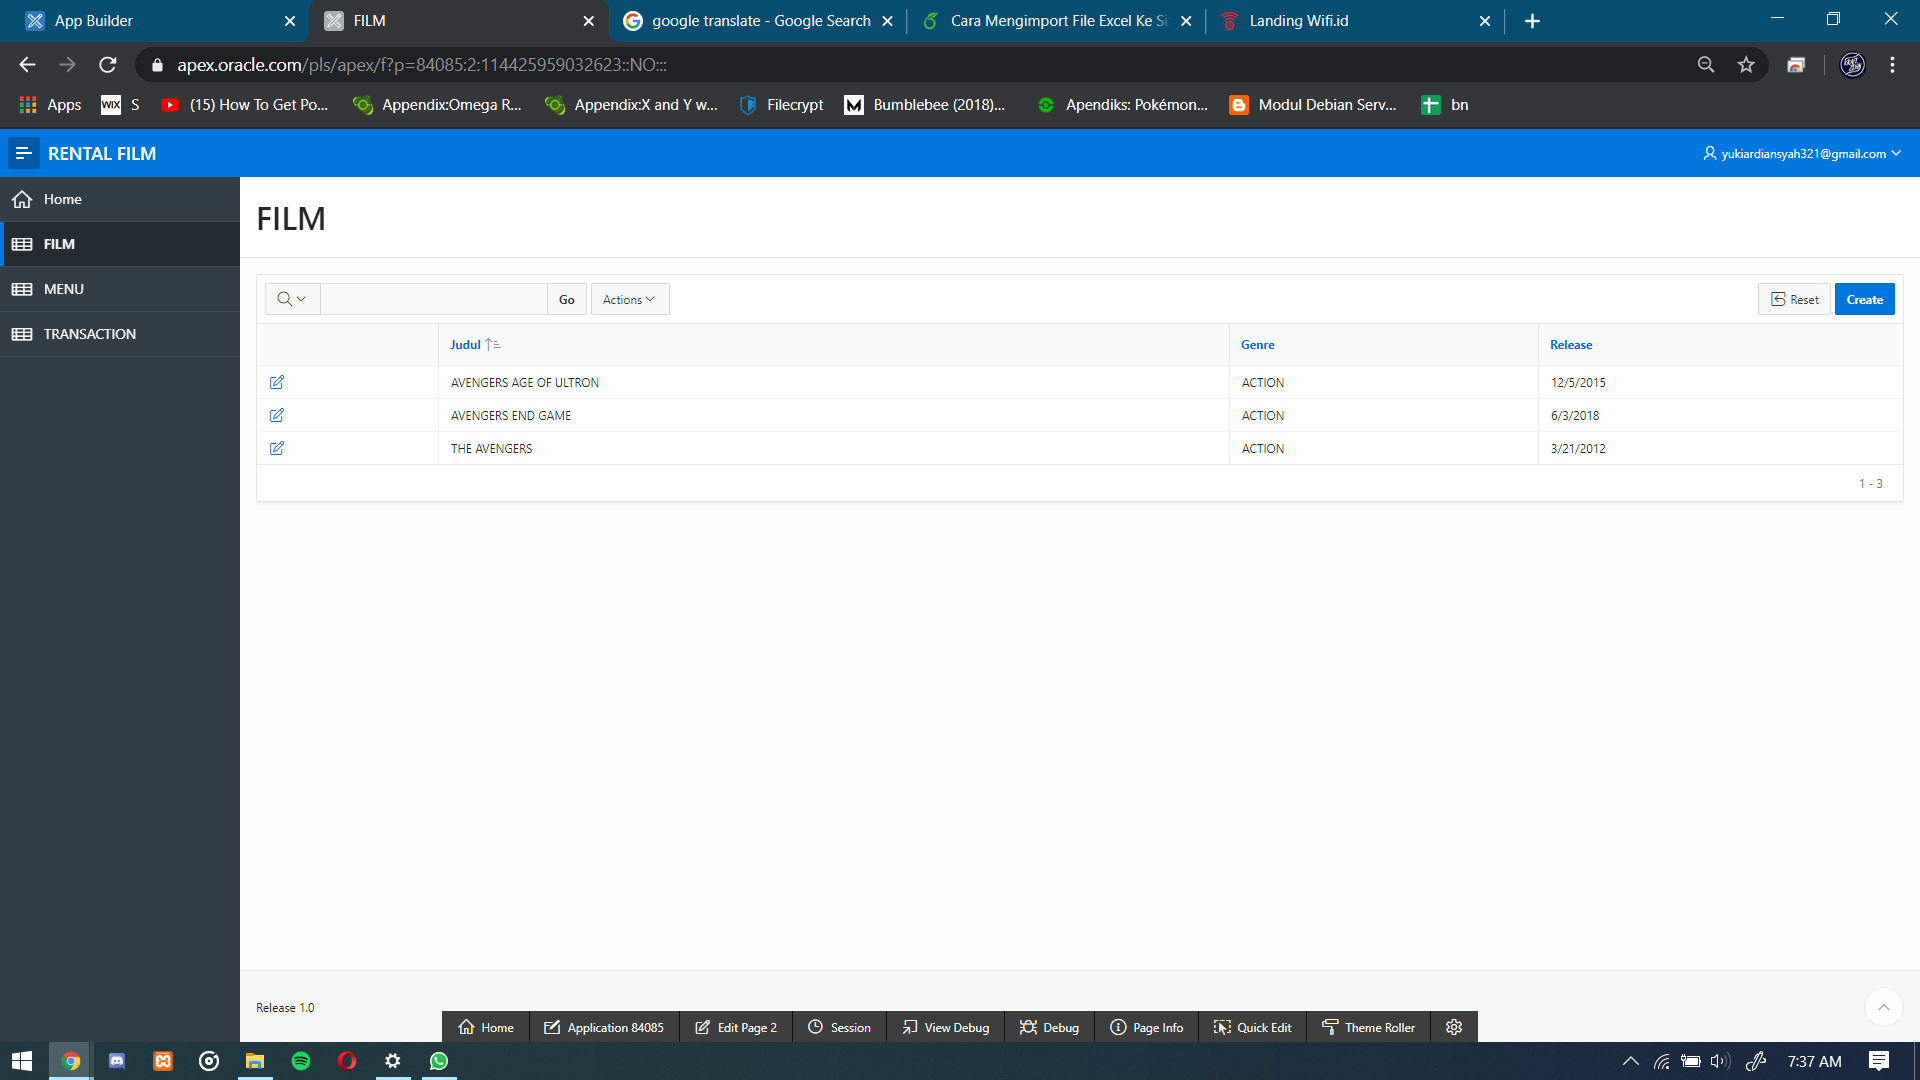
\includegraphics[scale=0.27]{figures/15.PNG}
        \caption{ready}
    \end{center}
\end{enumerate}
\section{Password username}
      
      \begin{enumerate}
      \item link https://apex.oracle.com/pls/apex/f?p=84085:2:114425959032623::NO:::
          \item workspace "YUKI"
          
          \item username "YUKIARDIANSYAH321@GMAIL.COM"
          
          \item password "shafaardi21"
      \end{enumerate}
      
       

\end{document}
